% \chapter{Đánh giá và Kiểm thử hệ thống}
% Tất cả quá trình kiểm thử hệ thống được nhóm tiến hành trên môi trường:
% \begin{itemize}
%     \item \textbf{Phiên bản mới nhất của ba trình duyệt web phổ biến hiện tại:}
%     \begin{itemize}
%         \item Google Chrome: Phiên bản 129.0.6668.90
%         \item Microsoft Edge: Phiên bản 129.0.2792.79
%         \item Brave: Phiên bản 1.66.110
%     \end{itemize}
%     \item \textbf{Máy chủ cơ sở dữ liệu:} PostgreSQL
%     \item \textbf{Hệ điều hành:} Windows 10, macOS
%     \item \textbf{Mạng:} Tốc độ download và upload được đo tại SpeedTest by Ookla, trang web đo tốc độ truy cập Internet và Ping nổi tiếng hiện nay, lần lượt là 372.34 Mbps (tương đương 46.5 MB/s) và 265.63 Mbps (tương đương 33.2 MB/s)
% \end{itemize}
% \section{Kiểm thử các yêu cầu chức năng}

% Kiểm thử các yêu cầu chức năng của quy trình mua sản phẩm
% \begin{longtable}{| m{4cm} | m{4cm} | m{4cm} | m{1.5cm} |}
%     \hline
%     \rowcolor{Gray}
%     \bf Tính năng & \bf Điều kiện & \bf Kết quả mong muốn & \bf Kết quả \\ 
%     \hline
%     A1. Hiển thị danh sách các sản phẩm & Truy cập trang chủ & Hiển thị danh sách các sản phẩm theo từng loại & Đạt  \\ 
%     \hline
%     A2. Thêm sản phẩm vào giỏ hàng & Truy cập trang hiển thị danh sách sản phẩm & Sản phẩm được thêm vào giỏ hàng & Đạt \\   
%     \hline
%     A3. Xóa sản phẩm khỏi giỏ hàng & Truy cập trang giỏ hàng & Sản phẩm được xóa khỏi giỏ hàng & Đạt \\   
%     \hline
%     A4. Cập nhật sản phẩm trong giỏ hàng & Truy cập trang giỏ hàng & Số lượng sản phẩm được cập nhật trong giỏ hàng & Đạt \\   
%     \hline
%     A5. Tạo đơn hàng mới & Tiến hành đặt hàng từ trang giỏ hàng & Đơn đặt hàng được tạo mới thành công và thông báo được gửi về cho khách hàng và chủ cửa hàng & Đạt \\   
%     \hline
%     \caption{\label{demo-table} Danh sách kiểm thử các tính năng quy trình mua sản phẩm}
% \end{longtable}

% Kiểm thử các yêu cầu chức năng của phần quản lý đơn hàng
% \begin{longtable}{| m{4cm} | m{4cm} | m{4cm} | m{1.5cm} |}
%     \hline
%     \rowcolor{Gray}
%     \bf Tính năng & \bf Điều kiện & \bf Kết quả mong muốn & \bf Kết quả \\ 
%     \hline    
%     B1. Xem danh sách đơn hàng & Truy cập trang quản lý đơn hàng trong kênh người bán & Hiển thị danh sách các đơn hàng & Đạt  \\ 
%     \hline
%     B2. Cập nhật trạng thái đơn hàng & Truy cập trang quản lý đơn hàng trong kênh người bán & Trạng thái đơn hàng được cập nhật thành công & Đạt  \\ 
%     \hline
%     B3. Hủy đơn hàng & Truy cập trang quản lý đơn hàng trong kênh người bán & Đơn hàng được hủy thành công & Đạt \\   
%     \hline
%     B4. Lấy thông tin chi tiết đơn hàng & Truy cập trang quản lý đơn hàng trong kênh người bán & Hiển thị chi tiết thông tin đơn hàng và thông tin người mua & Đạt \\   
%     \hline
%     B5. Tìm kiếm đơn hàng theo các tiêu chí & Truy cập trang quản lý đơn hàng trong kênh người bán & Hiện thị các đơn hàng phù hợp với tiêu chí tìm kiếm & Đạt \\   
%     \hline
%     \caption{\label{demo-table} Danh sách kiểm thử các tính năng phần quản lý đơn hàng}
% \end{longtable}

% Kiểm thử các yêu cầu chức năng của phần quản lý người dùng
% \begin{longtable}{| m{4cm} | m{4cm} | m{4cm} | m{1.5cm} |}
%     \hline
%     \rowcolor{Gray}
%     \bf Tính năng & \bf Điều kiện & \bf Kết quả mong muốn & \bf Kết quả \\ 
%     \hline
%     C1. Đăng ký tài khoản và mật khẩu mới & Nhập tên đăng nhập và mật khẩu chưa được đăng ký & Chuyển hướng về trang đăng nhập & Đạt  \\ 
%     \hline
%     C2. Đăng nhập bằng tài khoản và mật khẩu đúng & Nhập tên đăng nhập và mật khẩu đã đăng ký & Chuyển hướng về trang đang truy cập & Đạt  \\ 
%     \hline
%     C3. Đăng nhập bằng tài khoản, mật khẩu không hợp lệ & Nhập tên đăng nhập hoặc mật khẩu không đúng & Hiển thị thông báo lỗi & Đạt \\ 
%     \hline
%     C4. Đăng nhập bỏ trống tên đăng nhập hoặc mật khẩu & Không nhập tên đăng nhập hoặc mật khẩu & Hiển thị thông báo lỗi & Đạt \\   
%     \hline
%     \caption{\label{demo-table} Danh sách kiểm thử các tính năng phần quản lý người dùng}
% \end{longtable}
% \section{Đánh giá hệ thống}
% \subsection{Đánh giá hiệu suất}
% PageSpeed Insights là công cụ phân tích hiệu suất website do Google phát triển. 
% Nó cung cấp báo cáo chi tiết về tốc độ tải trang trên cả thiết bị di động và máy tính để bàn. 
% Công cụ này đánh giá nhiều yếu tố ảnh hưởng đến hiệu suất, bao gồm thời gian tải trang, tối ưu hóa hình ảnh, và tối ưu hóa mã nguồn. 
% PageSpeed Insights chấm điểm website từ 0 đến 100, trong đó điểm càng cao thể hiện hiệu suất càng tốt. 
% Website của nhóm đạt điểm khoảng 84 và đôi khi là 91, có thể coi là mức khá tốt. Trong quá trình phát triển, nhóm đã cải thiện và tối ưu hóa trang web để đạt được điểm số như vậy.
% \begin{figure}[H]
%     \centering
%     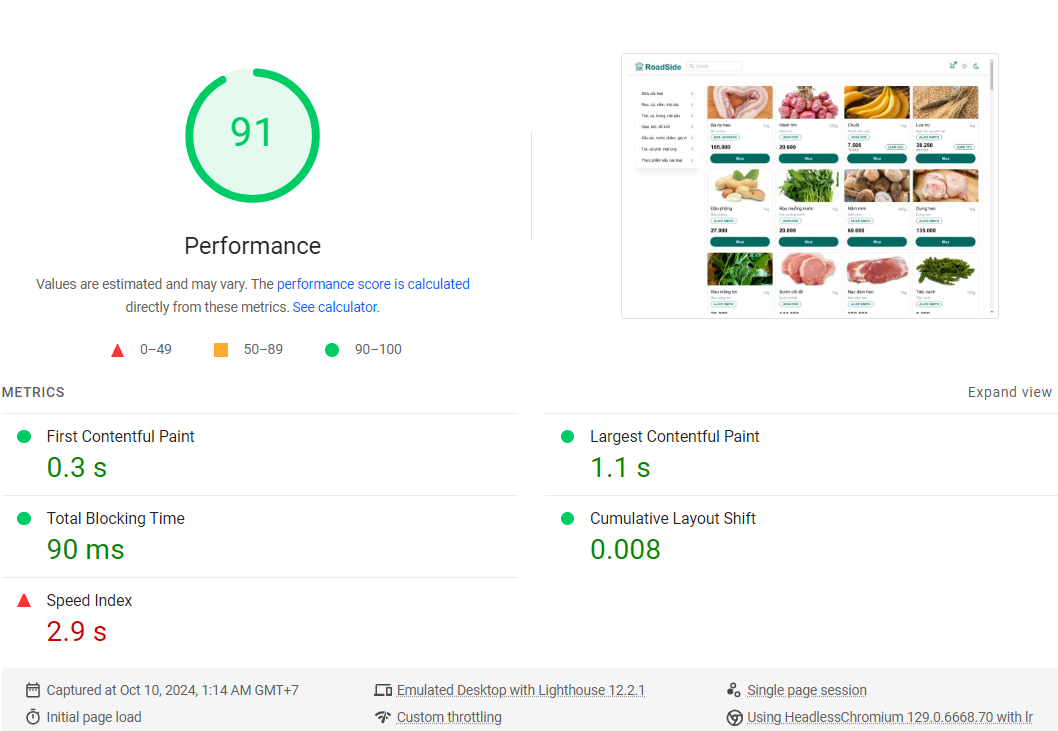
\includegraphics[width=\linewidth] {Images/UI/performance.png}
%     \vspace{1em}
%     \caption{Đánh giá hiệu suất website trên PageSpeed Insights}
% \end{figure}

% Như có thể thấy, phải mất khoảng 2,5 đến 2,9 giây để tải đầy đủ trang web, tuy nhiên, con số này có thể được cải thiện bằng cách tối ưu hóa các chiến lược sau theo gợi ý của Page Speed ​​Insight.
% \begin{itemize}
%     \item Thay đổi kích thước hình ảnh phù hợp
%     \item Giảm thiểu những đoạn mã JavaScript không sử dụng
%     \item Mã hóa hình ảnh
%     \item Giảm thiểu những đoạn mã CSS không sử dụng
% \end{itemize}